\section{设计结果}

\subsection{设计交付物说明}
\textcolor{black}{设计交付物分为两次提交,第一次提交代码相关资料。解压后可以获得一个以学号-姓名-11-submit 命名的文件夹。文件夹下的目录树如图所示:}

\begin{figure}[htbp]
    \centering
    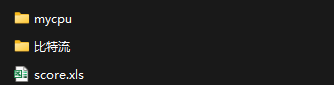
\includegraphics[width=\textwidth]{image/fileconstruct.png}
    \caption{文件结构}
\end{figure}
    
\textcolor{black}{bit 文件夹下存放了一个.bit 文件;perf.bit 是在soc\_axi\_perf工程下生成的性能测试比特流文件。
mycpu 文件夹下存放了我们项目工程的源代码,cache 文件夹存放的是 i\_cache 与d\_cache 以及 bridge\_1x2 与 bridge\2x1。controller 文件夹存放的是控制模块包括 aludec 与maindec。datapath 文件夹包括数据通路 datapath 与 hazard。utils 是数据通路中的模块。将源代码加入对应工程的 rtl 文件夹中,即可进行仿真、综合、实现等一系列操作。score.xls 文件记录了我们的性能测试得分。第二次提交的文件为课程设计报告,命名方式与第一次提交相同。
}

\subsection{设计演示结果} 
\subsubsection{功能测试结果}
\textcolor{black}{功能测试点全部通过}
\textcolor{black}{bitcount 结果}\\
\begin{figure}[htbp]
    \centering
    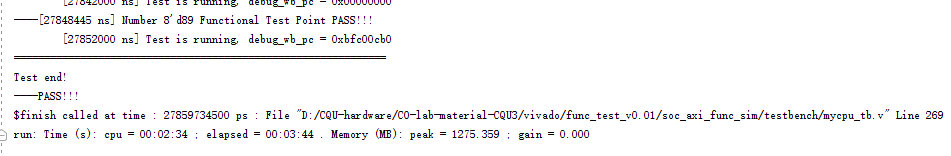
\includegraphics[width=\textwidth]{image/functest.png}
    \caption{功能测试通过}
\end{figure}

\subsubsection{性能测试结果}
\textcolor{black}{包括仿真图与实际上板图}\\
\textcolor{black}{(1)bitcount 结果}\\
\begin{figure}[h]
    \centering
    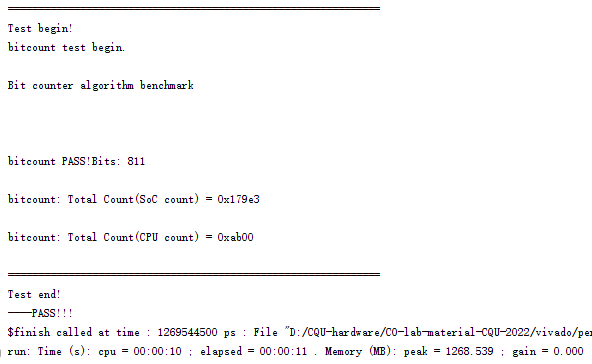
\includegraphics[width=0.9\textwidth]{image/bitcountS.png}
    \caption{bitcount仿真}
\end{figure}

\begin{figure}[h]
    \centering
    \rotatebox{90}{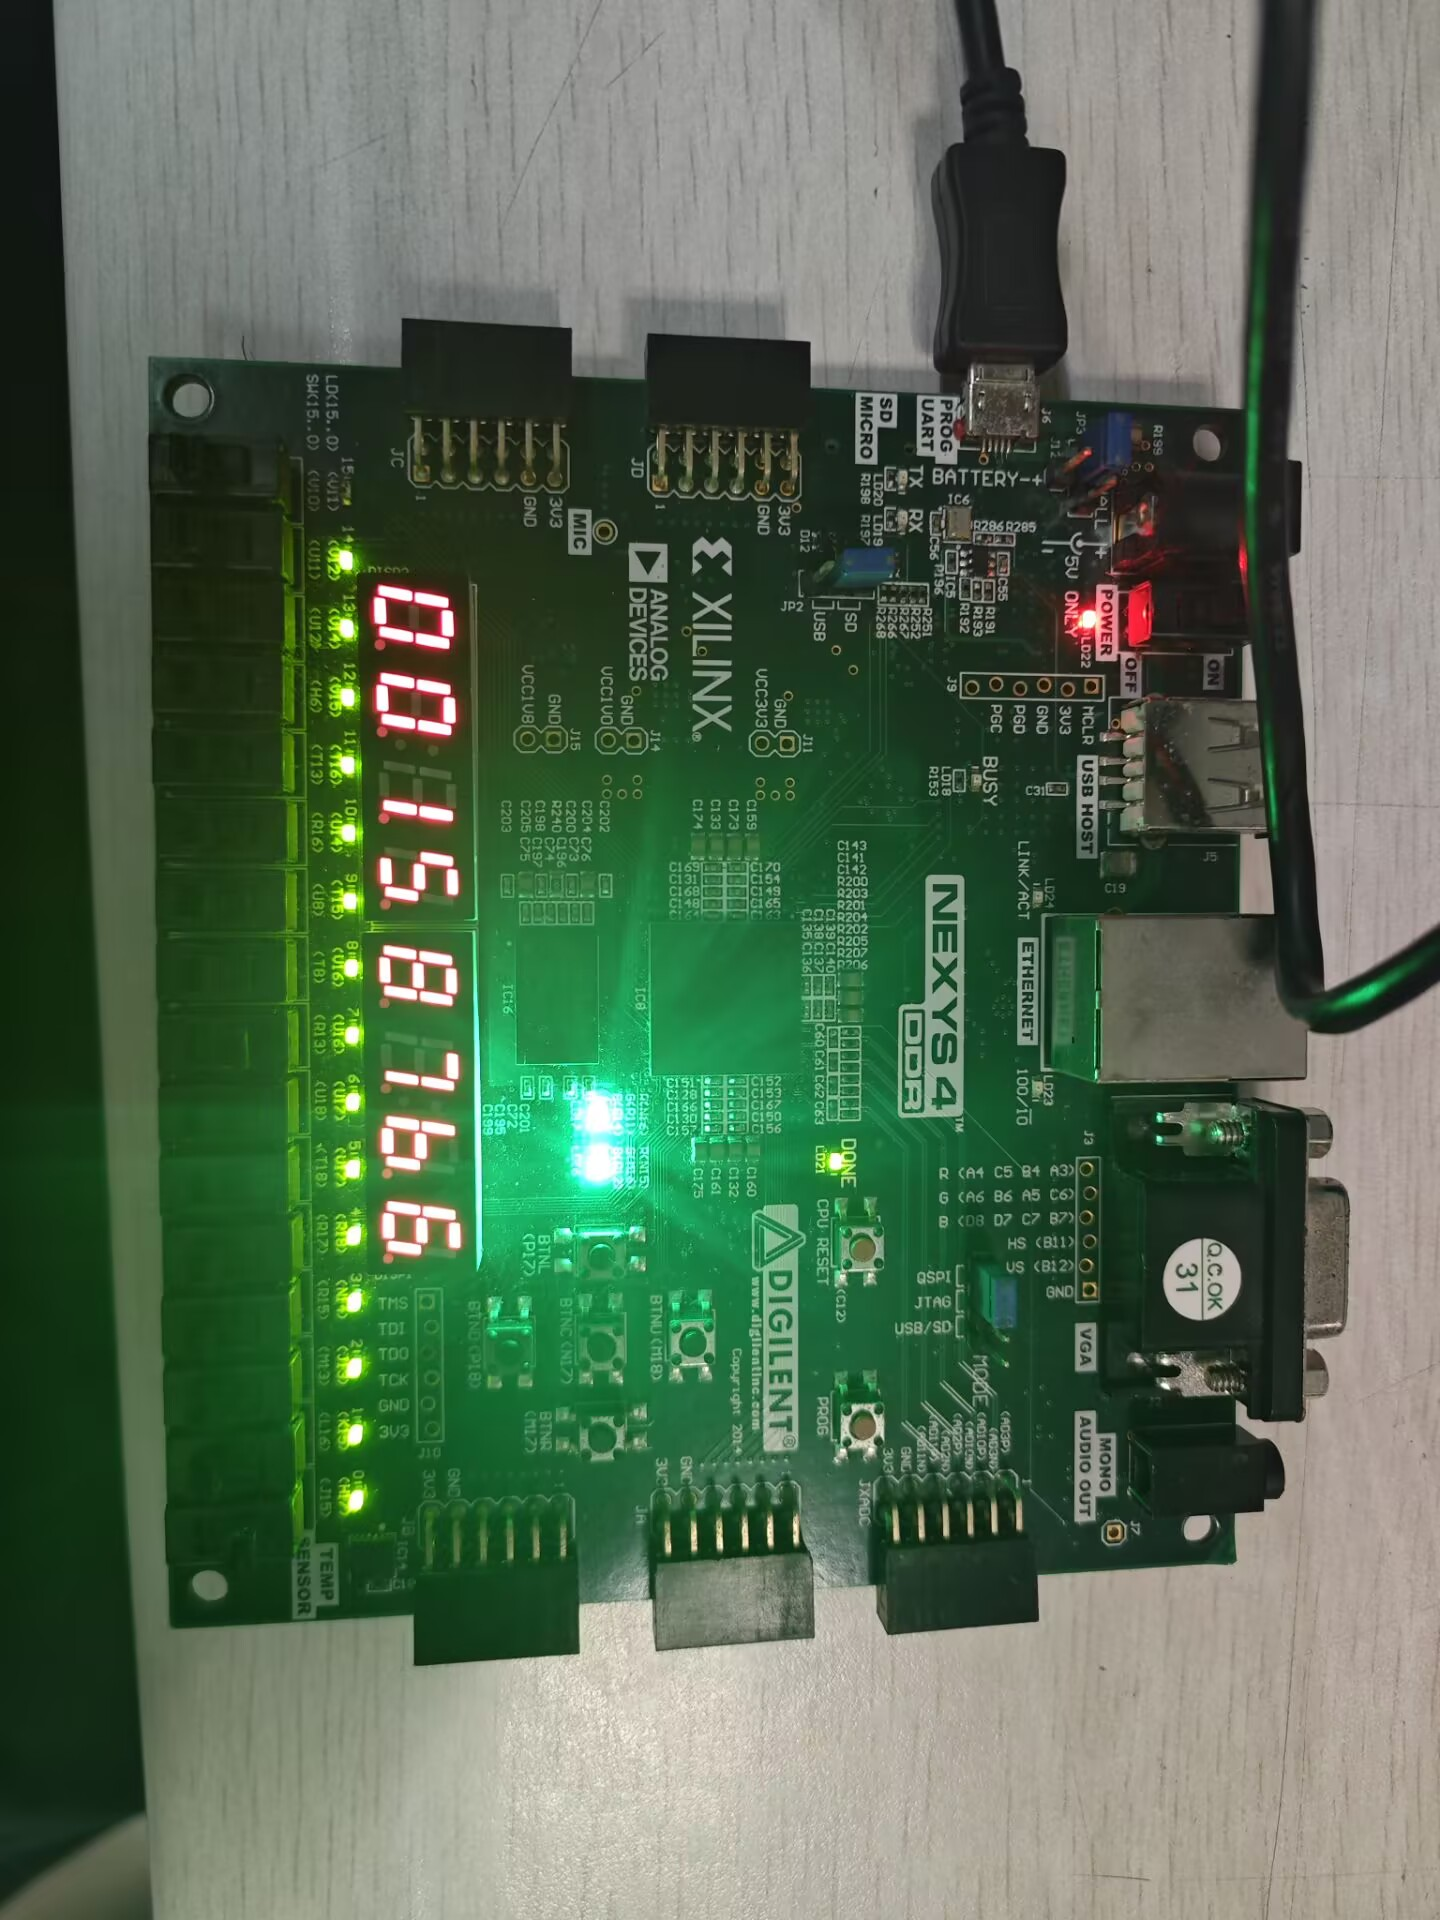
\includegraphics[width=0.5\textwidth]{image/bitcountB.jpg}}
    \caption{bitcount上板}
\end{figure}

\newpage
\textcolor{black}{(2)bubble\_sort 结果}\\
\begin{figure}[h]
    \centering
    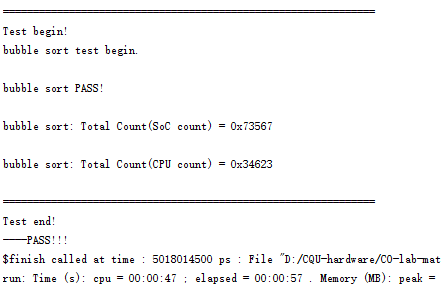
\includegraphics[width=0.9\textwidth]{image/bubbleS.png}
    \caption{bubble\_sort仿真}
\end{figure}

\begin{figure}[h]
    \centering
    \rotatebox{0}{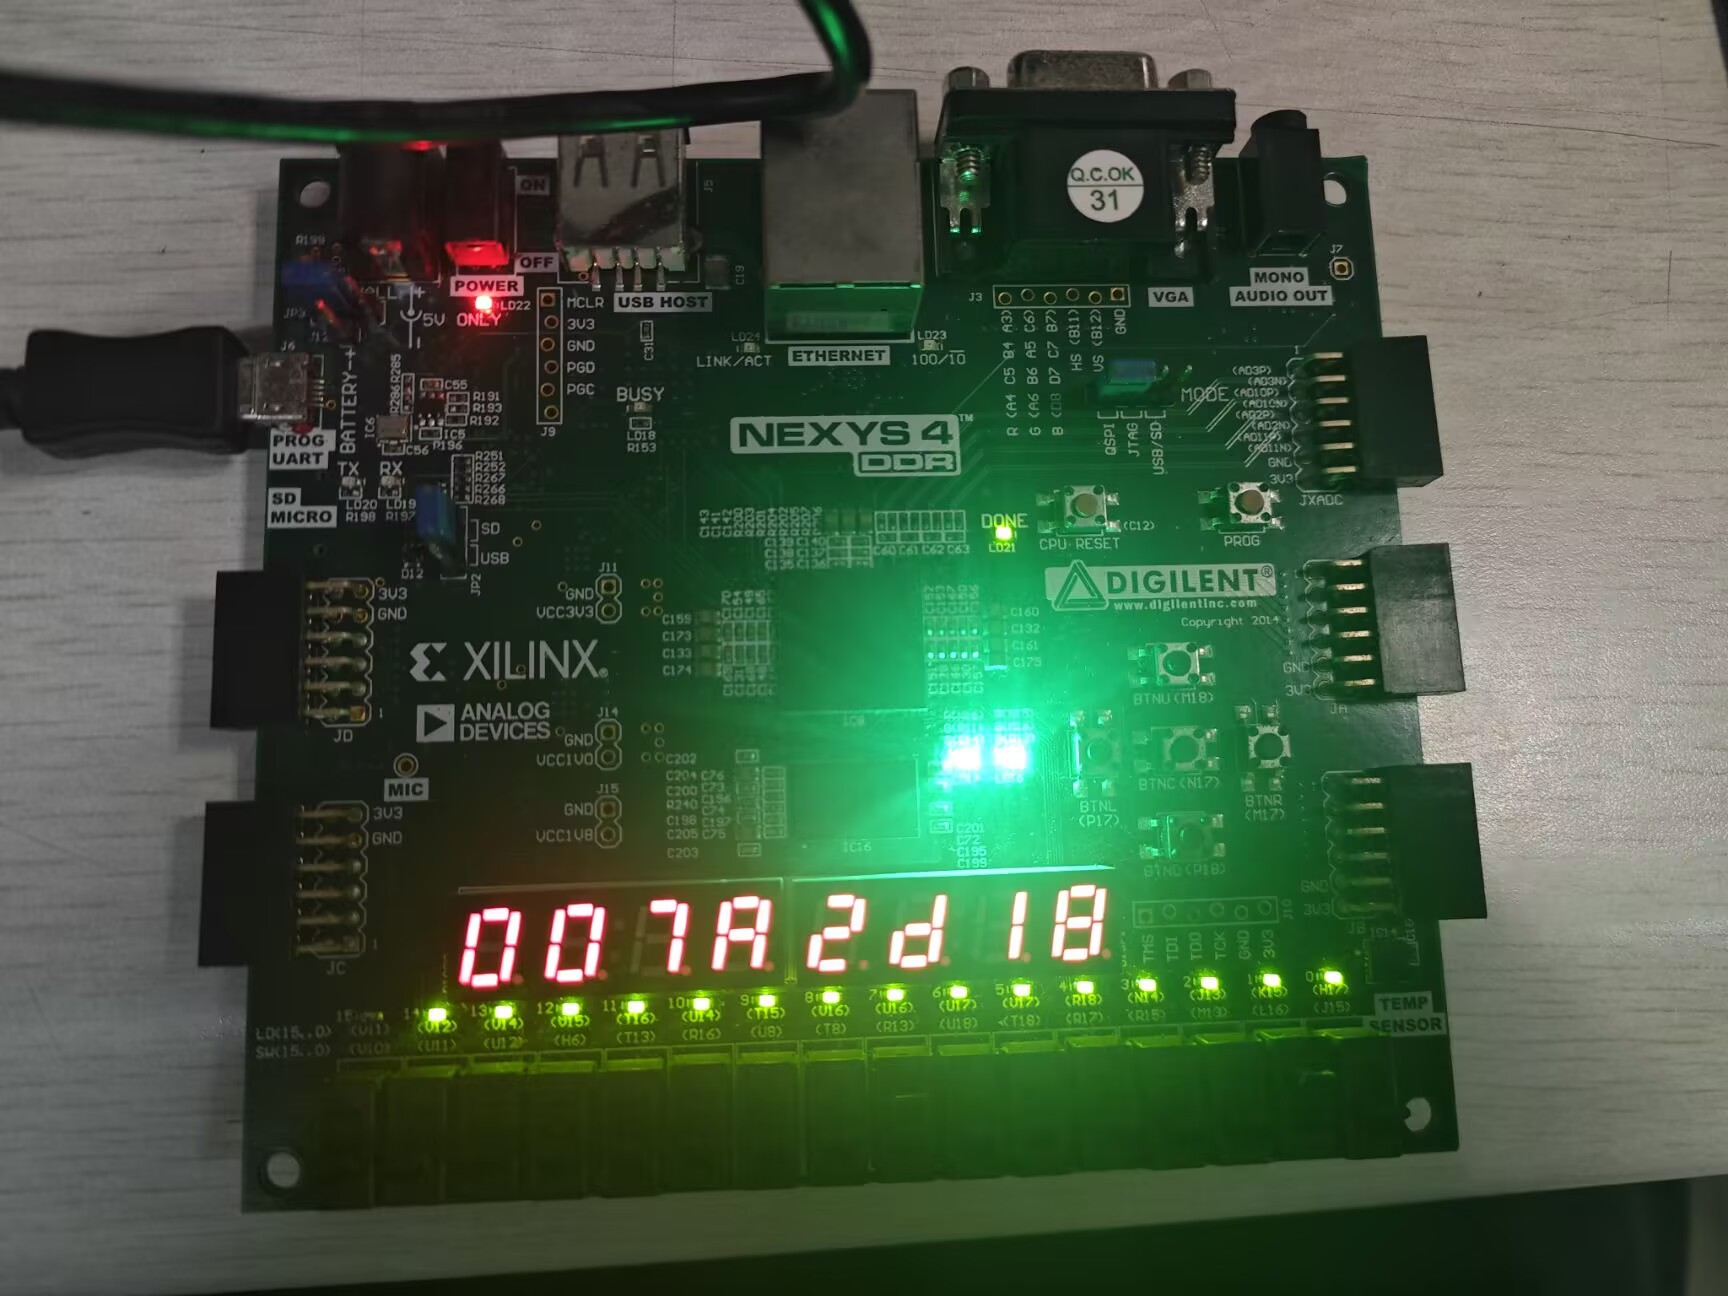
\includegraphics[width=0.5\textwidth]{image/bubblesB.jpg}}
    \caption{bubble\_sort上板}
\end{figure}

\newpage
\textcolor{black}{(3)coremark 结果}\\
\begin{figure}[htbp]
    \centering
    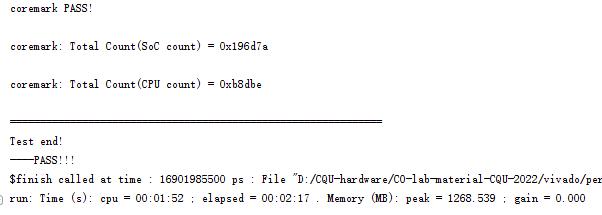
\includegraphics[width=0.9\textwidth]{image/coreS.png}
    \caption{coremark仿真}
\end{figure}

\begin{figure}[htbp]
    \centering
    \rotatebox{90}{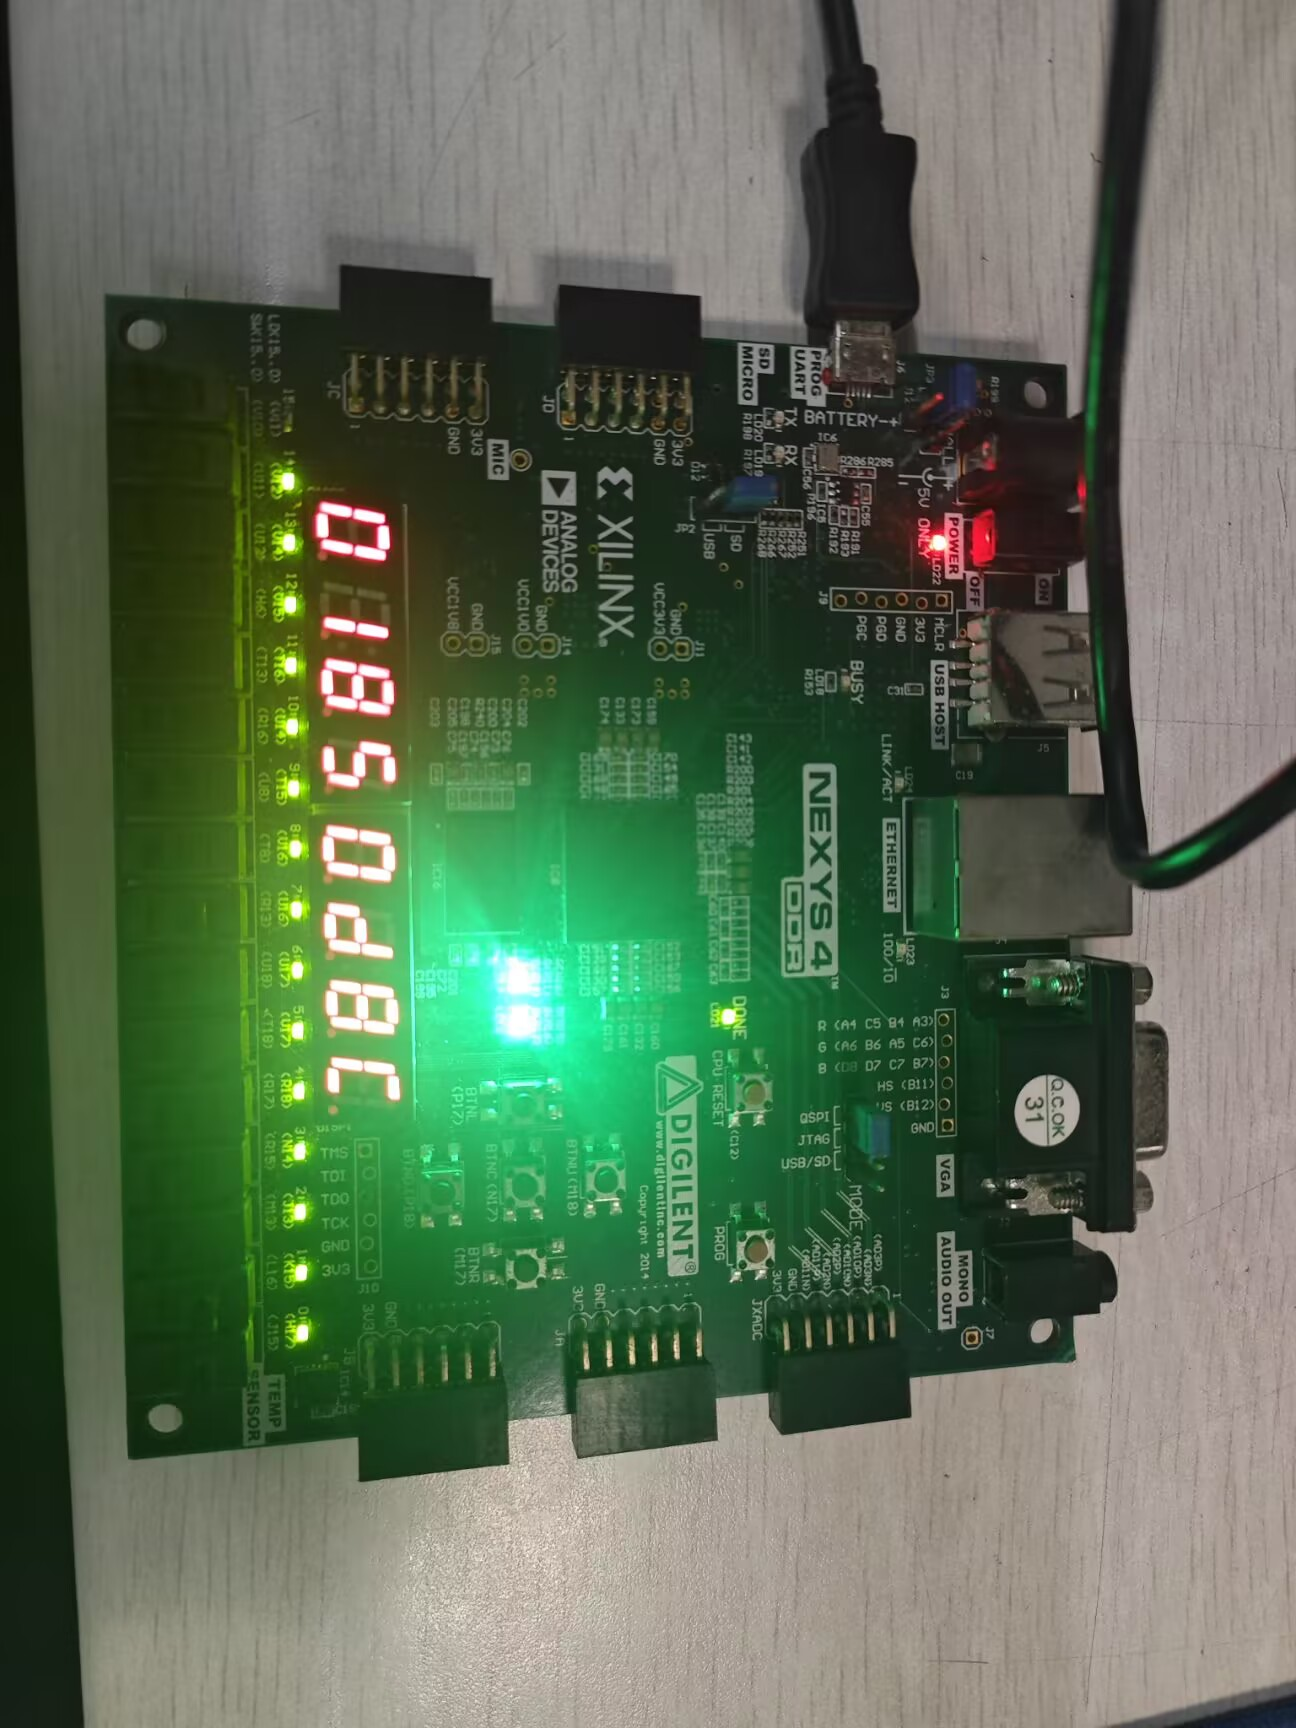
\includegraphics[width=0.5\textwidth]{image/coremarkB.jpg}}
    \caption{coremark上板}
\end{figure}

\newpage
\textcolor{black}{(4)crc32 结果}\\
\begin{figure}[htbp]
    \centering
    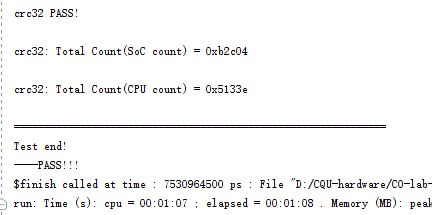
\includegraphics[width=0.9\textwidth]{image/crc32S.png}
    \caption{crc32仿真}
\end{figure}

\begin{figure}[htbp]
    \centering
    \rotatebox{90}{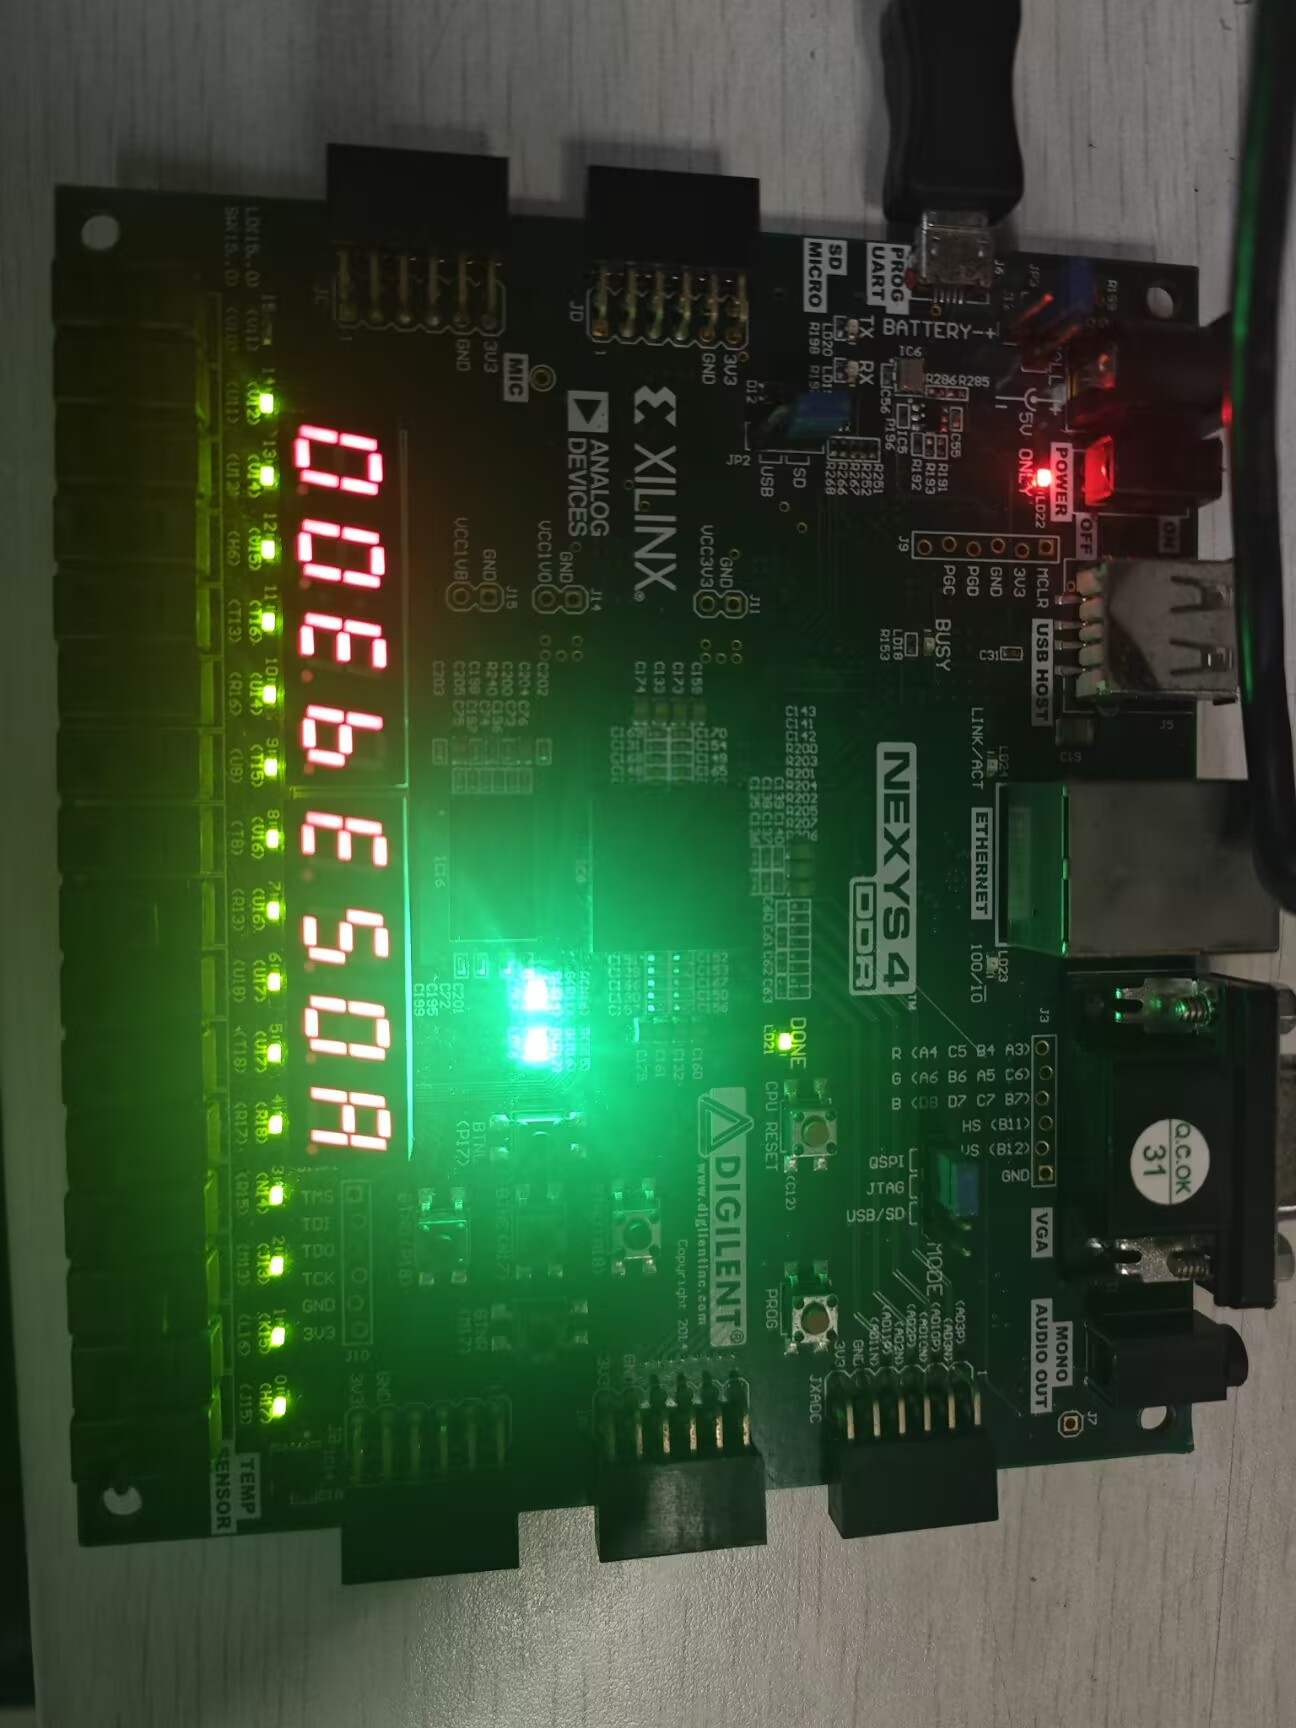
\includegraphics[width=0.5\textwidth]{image/crcB.jpg}}
    \caption{crc32上板}
\end{figure}

\newpage
\textcolor{black}{(5)dhrystone 结果}\\
\begin{figure}[htbp]
    \centering
    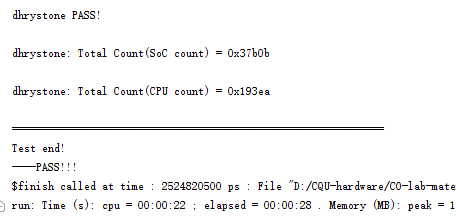
\includegraphics[width=0.9\textwidth]{image/dhtyS.png}
    \caption{dhry仿真}
\end{figure}

\begin{figure}[htbp]
    \centering
    \rotatebox{90}{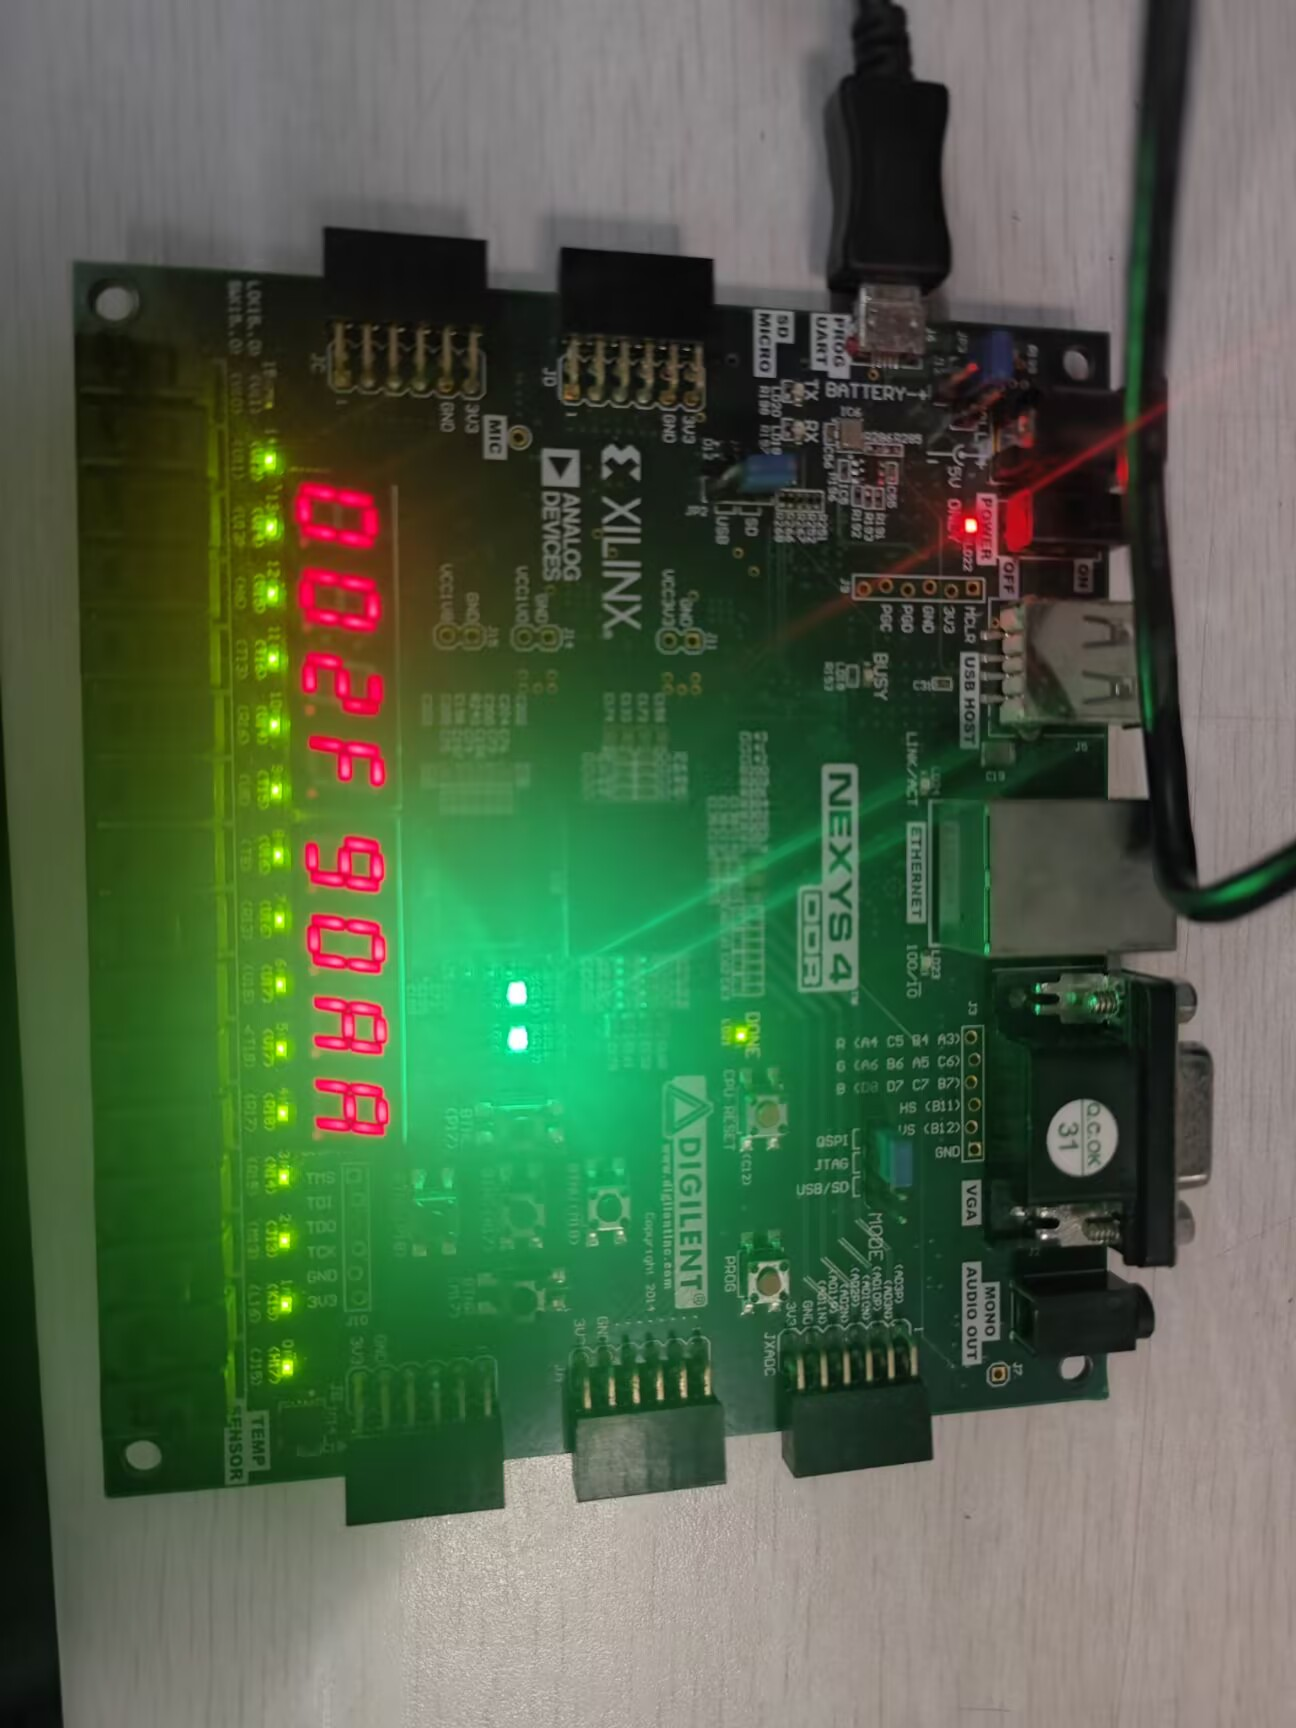
\includegraphics[width=0.5\textwidth]{image/dhryB.jpg}}
    \caption{dhry上板}
\end{figure}

\newpage
\textcolor{black}{(6)quick\_sort 结果}\\
\begin{figure}[htbp]
    \centering
    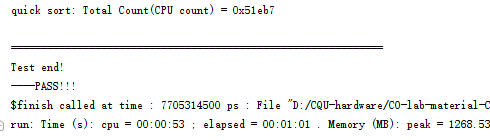
\includegraphics[width=0.9\textwidth]{image/quicksortS.png}
    \caption{quicksort仿真}
\end{figure}

\begin{figure}[htbp]
    \centering
    \rotatebox{0}{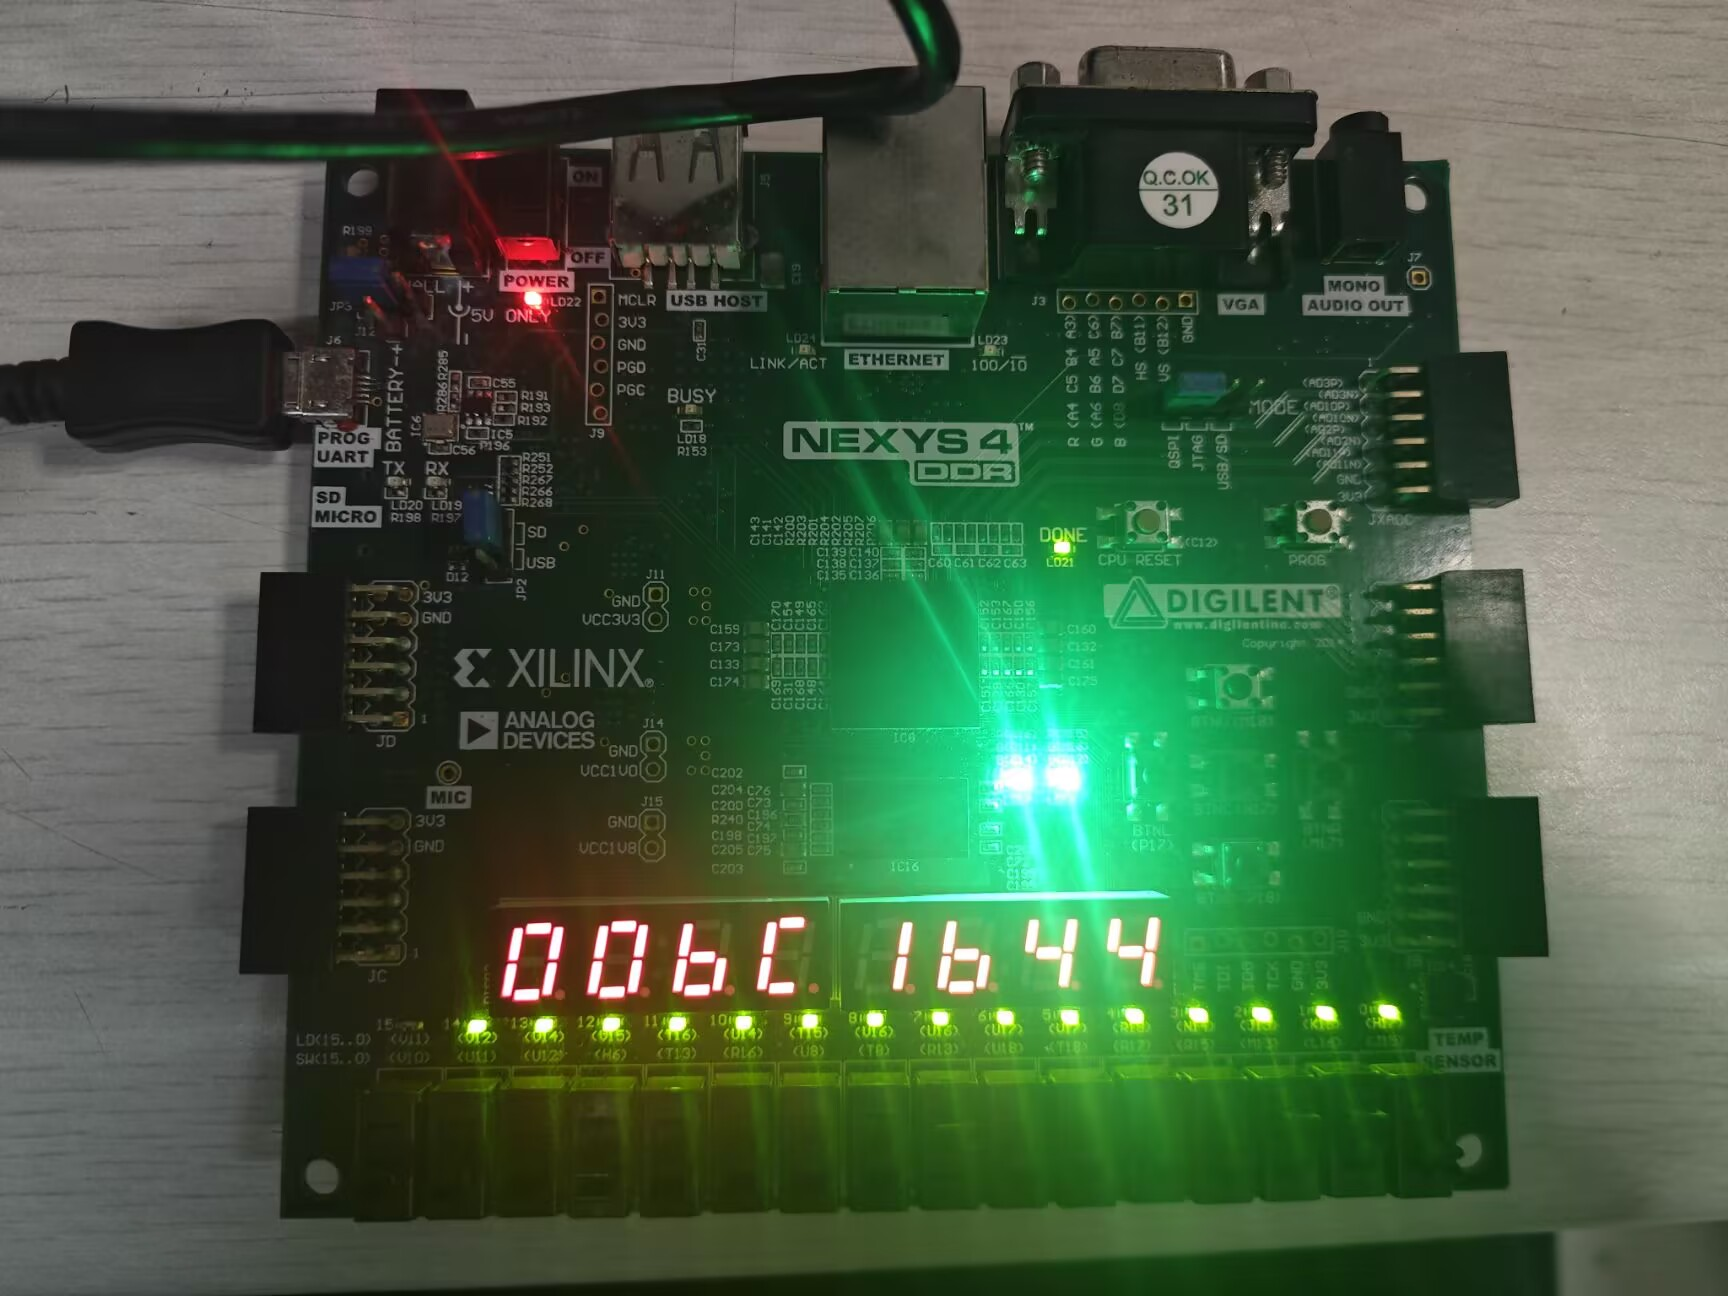
\includegraphics[width=0.5\textwidth]{image/quicksortB.jpg}}
    \caption{quicksort上板}
\end{figure}

\newpage
\textcolor{black}{(7)select\_sort 结果}\\
\begin{figure}[htbp]
    \centering
    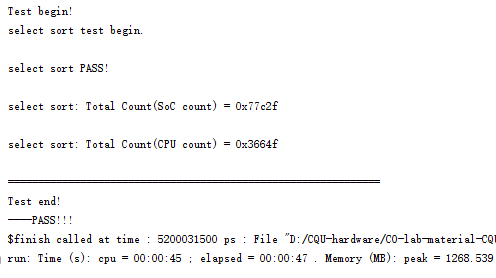
\includegraphics[width=0.9\textwidth]{image/selectsortS.png}
    \caption{selectsort仿真}
\end{figure}

\begin{figure}[htbp]
    \centering
    \rotatebox{90}{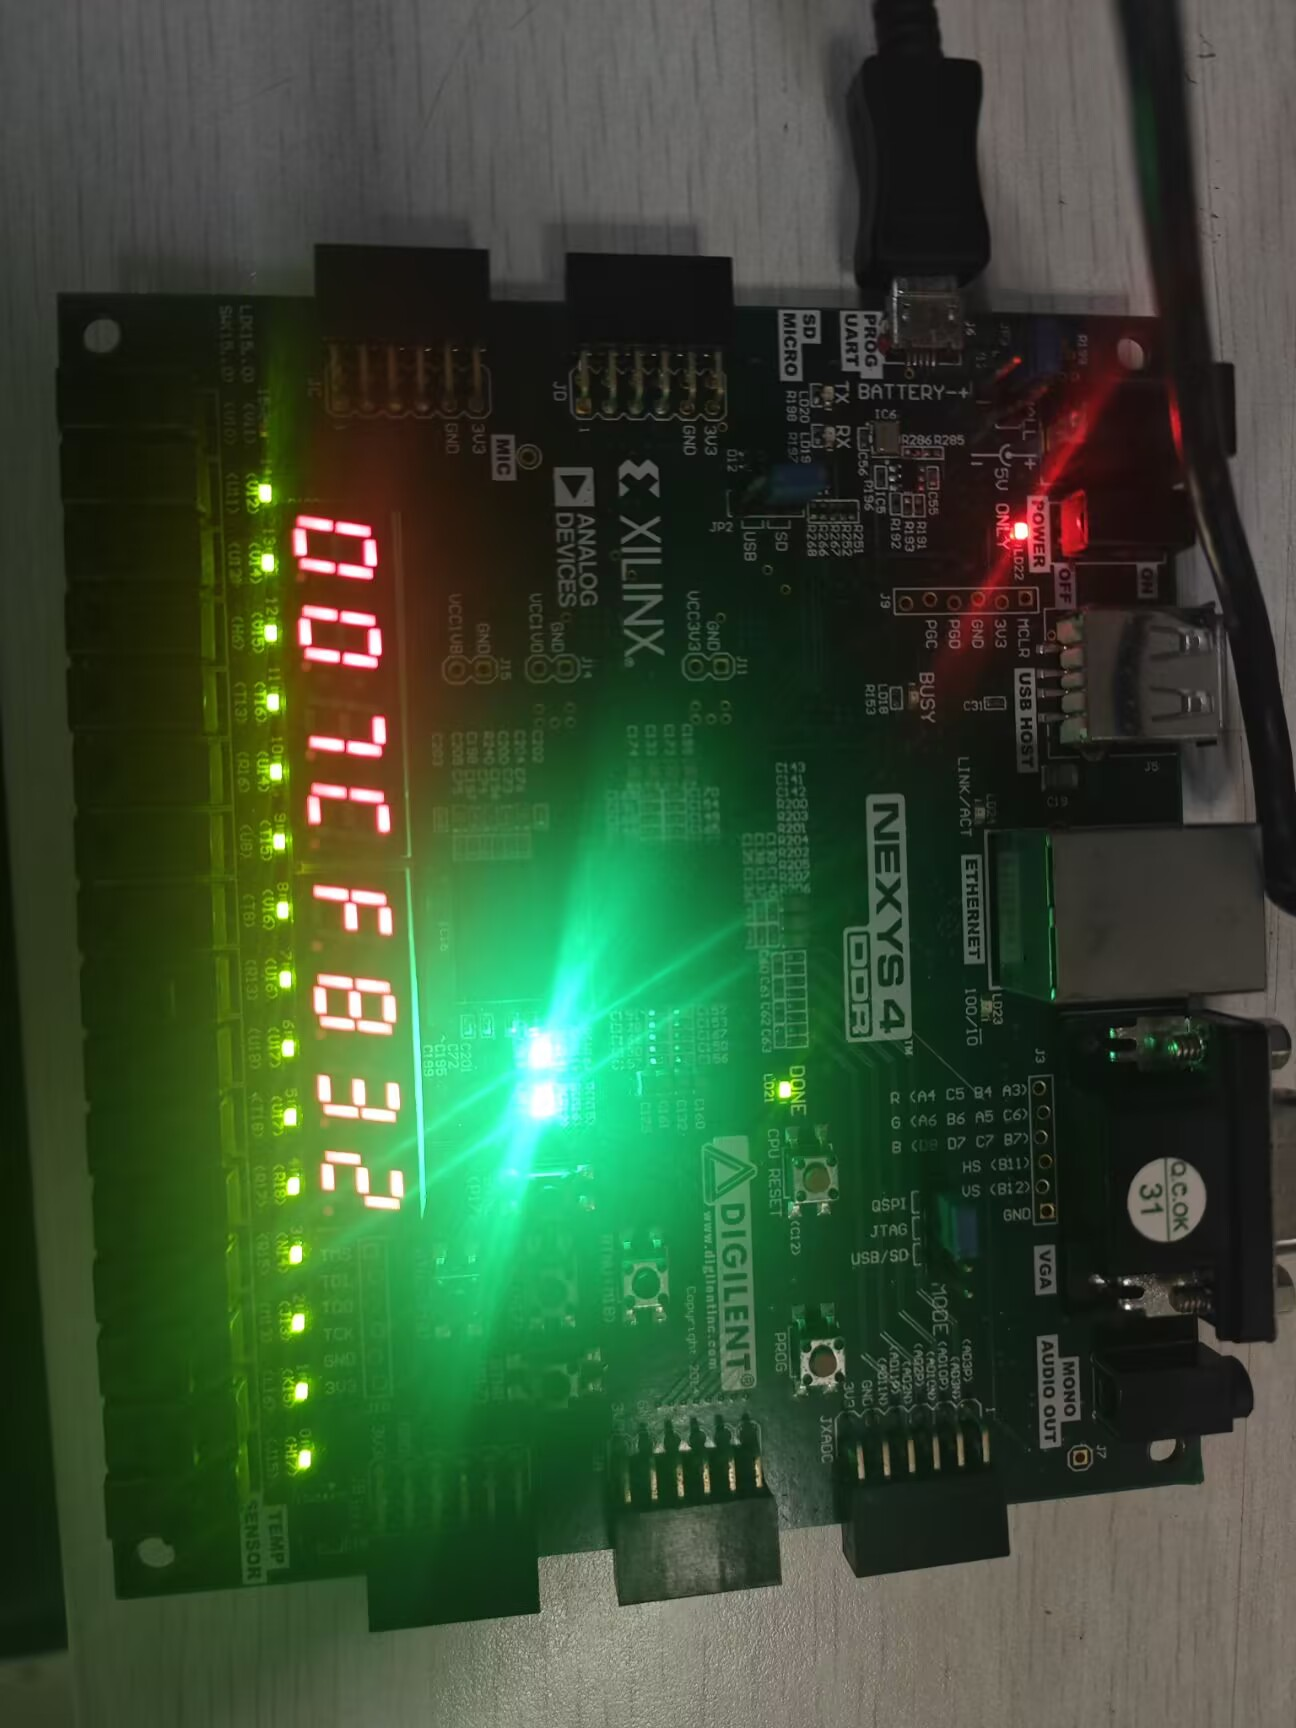
\includegraphics[width=0.5\textwidth]{image/selectsortB.jpg}}
    \caption{selectsort上板}
\end{figure}

\newpage
\textcolor{black}{(8)sha 结果}\\
\begin{figure}[htbp]
    \centering
    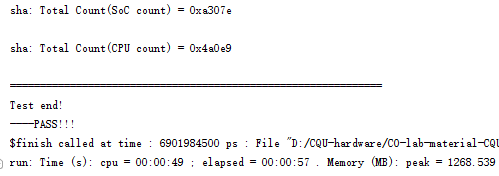
\includegraphics[width=0.9\textwidth]{image/shaS.png}
    \caption{sha仿真}
\end{figure}

\begin{figure}[htbp]
    \centering
    \rotatebox{90}{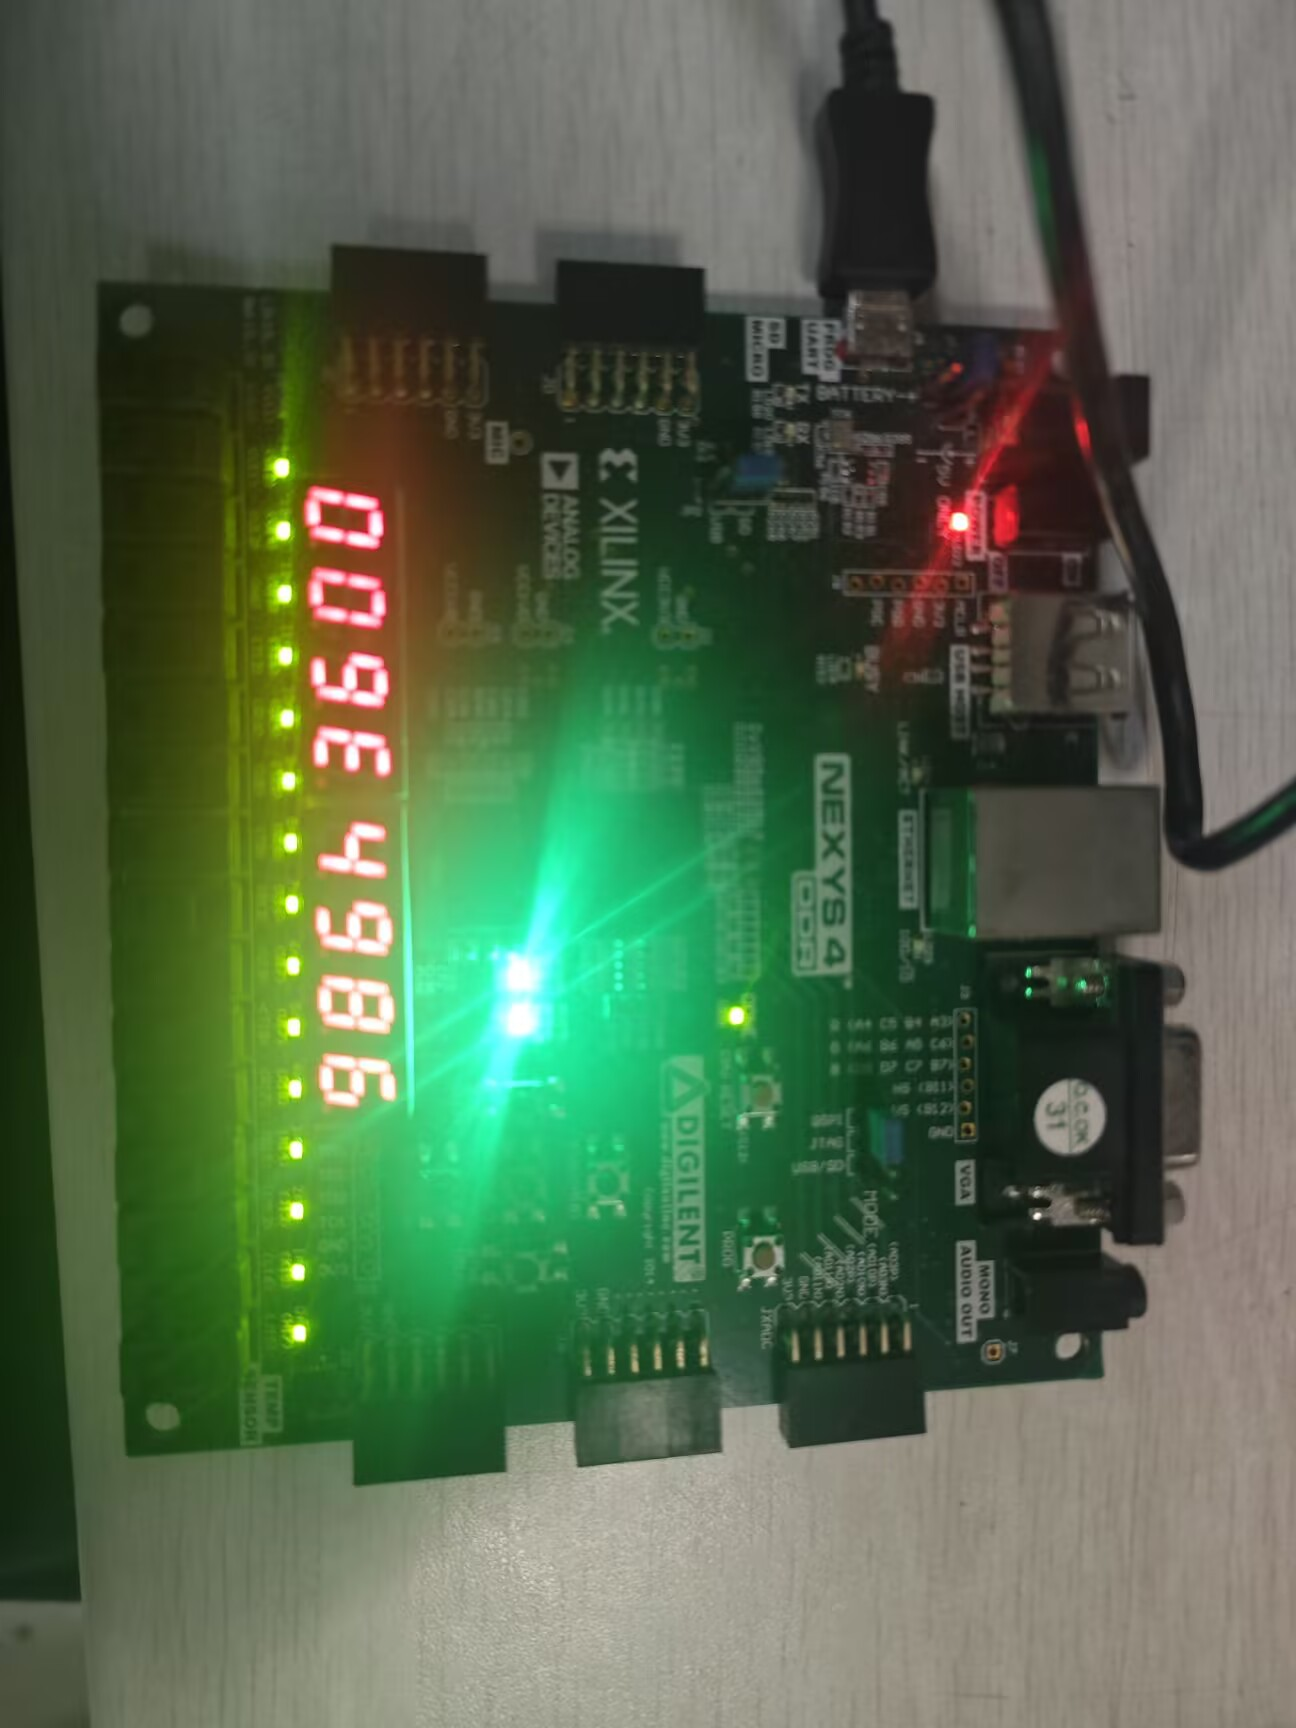
\includegraphics[width=0.5\textwidth]{image/shaB.jpg}}
    \caption{sha上板}
\end{figure}

\newpage
\textcolor{black}{(9)stream\_copy 结果}\\
\begin{figure}[htbp]
    \centering
    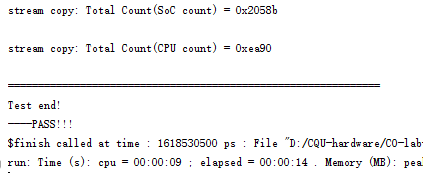
\includegraphics[width=0.9\textwidth]{image/streamcopyS.png}
    \caption{streamcopy仿真}
\end{figure}

\begin{figure}[htbp]
    \centering
    \rotatebox{90}{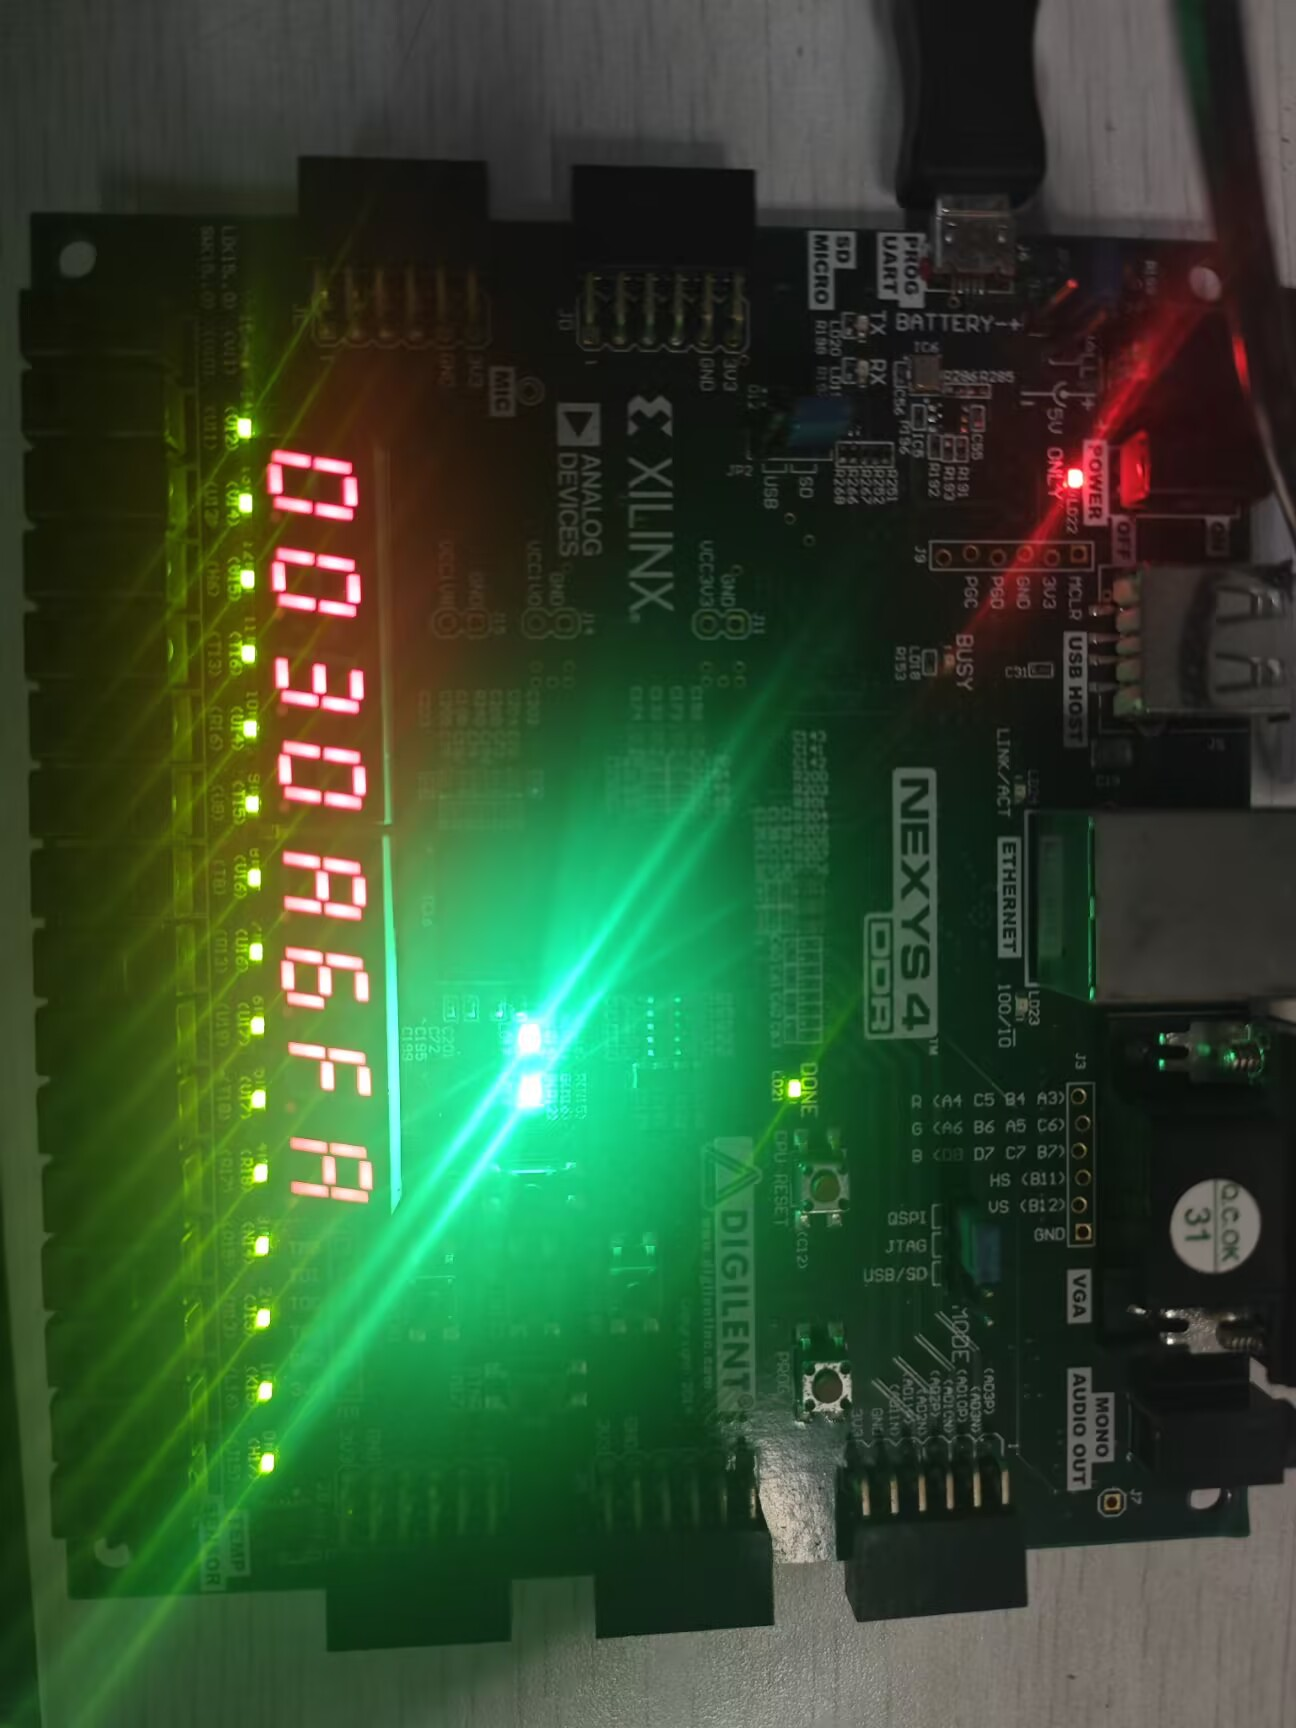
\includegraphics[width=0.5\textwidth]{image/streamcopyB.jpg}}
    \caption{streamcopy上板}
\end{figure}

\newpage
\textcolor{black}{(10)stringsearch 结果}\\
\begin{figure}[htbp]
    \centering
    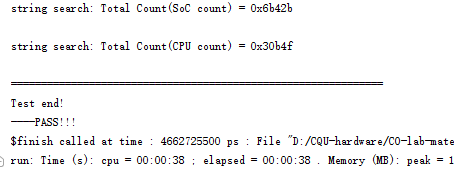
\includegraphics[width=0.9\textwidth]{image/stringsearchS.png}
    \caption{stringsearch仿真}
\end{figure}

\begin{figure}[htbp]
    \centering
    \rotatebox{90}{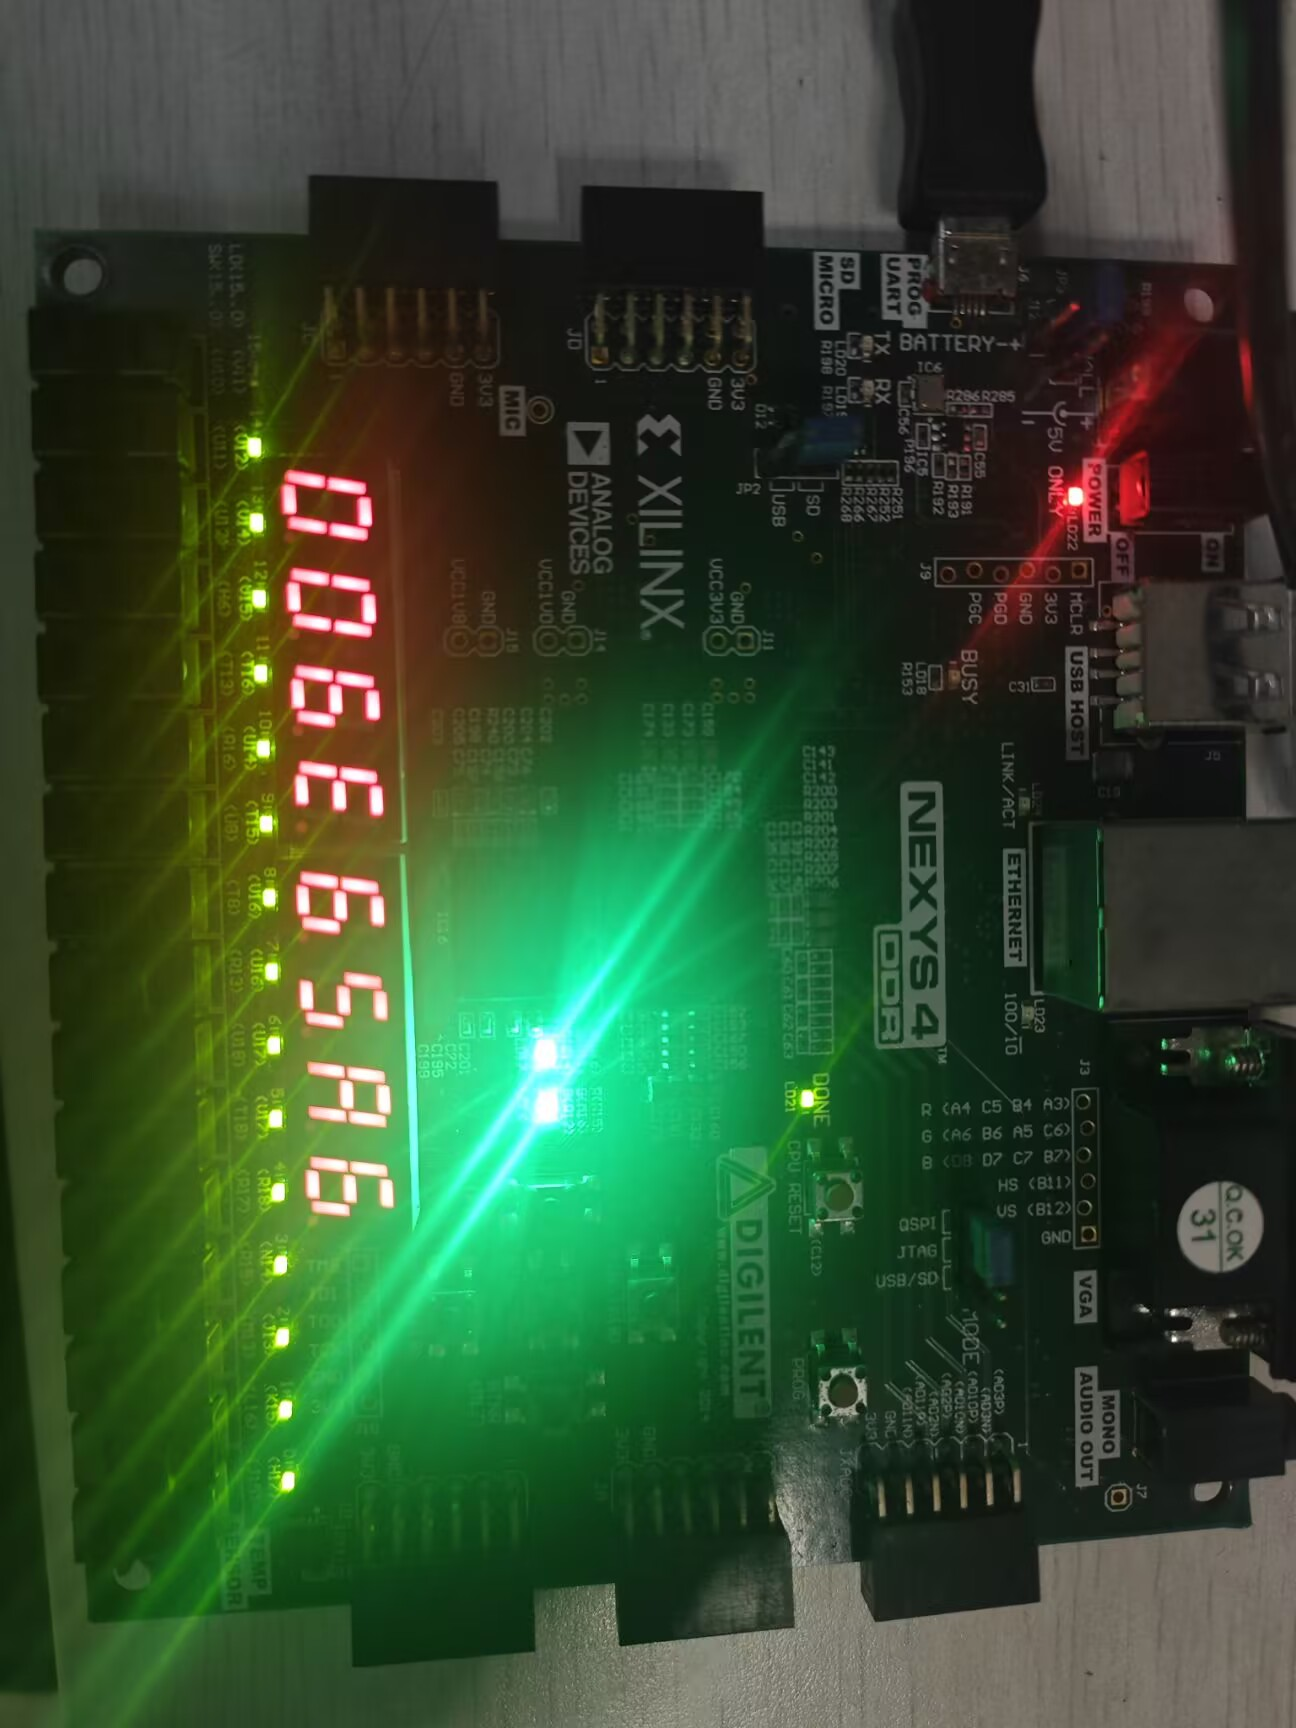
\includegraphics[width=0.5\textwidth]{image/stringsearchB.jpg}}
    \caption{stringsearch上板}
\end{figure}
